%%%%%%%%%%%%%%%%%%%MAIN_OPTIONS%%%%%%%%%%%%%%%%%%%
\documentclass[a4paper, 14pt]{article}

%% Работа с русским языком
\usepackage{cmap}					% поиск в PDF
\usepackage{hyperref}				% гиперссылки
\usepackage[warn]{mathtext} 		% русские буквы в формулах
\usepackage[T2A]{fontenc}			% кодировка
\usepackage[utf8]{inputenc}			% кодировка исходного текста
\usepackage[english,russian]{babel}	% локализация и переносы

%% Дополнительная работа с математикой
\usepackage{amsfonts,amssymb,amsthm,mathtools} % AMS
\usepackage{amsmath}
\usepackage{icomma} % "Умная" запятая: $0,2$ --- число, $0, 2$ --- перечисление

%% Номера формул
%\mathtoolsset{showonlyrefs=true} % Показывать номера только у тех формул, на которые есть \eqref{} в тексте.

%%FONTS_Packadges
\usepackage{euscript} % Шрифт Евклид
\usepackage{mathrsfs} % Красивый матшрифт

%% Свои команды
\DeclareMathOperator{\sgn}{\mathop{sgn}}

%% Перенос знаков в формулах (по Львовскому)
\newcommand*{\hm}[1]{#1\nobreak\discretionary{}
	{\hbox{$\mathsurround=0pt #1$}}{}}

%%% Работа с картинками
\usepackage{graphicx}  % Для вставки рисунков
\graphicspath{{pictures/}{images2/}}  % папки с картинками
\setlength\fboxsep{3pt} % Отступ рамки \fbox{} от рисунка
\setlength\fboxrule{1pt} % Толщина линий рамки \fbox{}
\usepackage{wrapfig} % Обтекание рисунков и таблиц текстом
\usepackage[section]{placeins}
\usepackage{subcaption}

%% Работа с таблицами
\usepackage{array,tabularx,tabulary,booktabs} % Дополнительная работа с таблицами
\usepackage{longtable}  % Длинные таблицы
\usepackage{multirow} % Слияние строк в таблице

%%Links
\hypersetup{
	colorlinks=true,
	linkcolor=black,
	filecolor=magenta,      
	urlcolor=blue,
}

%%% Программирование
\usepackage{etoolbox} % логические операторы

%%% Страница
\usepackage{extsizes} % Возможность сделать 14-й шрифт
\usepackage{geometry} % Простой способ задавать поля
\geometry{top=25mm}
\geometry{bottom=35mm}
\geometry{left=20mm}
\geometry{right=20mm}
\usepackage{indentfirst}
%
\usepackage{fancyhdr} % Колонтитулы
\pagestyle{fancy}
\renewcommand{\headrulewidth}{0mm}  % Толщина линейки, отчеркивающей верхний колонтитул
%\lfoot{Нижний левый}
%\rfoot{Нижний правый}
%\rhead{Верхний правый}
%\chead{Верхний в центре}
%\lhead{Верхний левый}
% \cfoot{Нижний в центре} % По умолчанию здесь номер страницы

\usepackage{setspace} % Интерлиньяж
%\onehalfspacing % Интерлиньяж 1.5
%\doublespacing % Интерлиньяж 2
%\singlespacing % Интерлиньяж 1

\usepackage{multicol,caption}

\newenvironment{Figure}
{\par\medskip\noindent\minipage{\linewidth}}
{\endminipage\par\medskip}

\usepackage{enumitem}
\usepackage{amssymb}
\usepackage{xcolor}
%%% Зачеркнутый текст
\usepackage[normalem]{ulem}
\usepackage{xurl}



\begin{document}

	\title{		\textbf{\textit{Победит \#398}} 
		
	Сбор геометрии регионов связ. в-ва}

	\author{$Е.П. Константинова^1, Д.Г. Каграманян^2, Б.Б. Страумал^3, Л.Н. Щур^4$}
	\date{\today}
	\maketitle

	\hfill
	\begin{minipage}{1\textwidth}
			\flushleft
		$^1$исследователь,lizaconst@icloud.com \\
	    $^2$исследователь,dgkagramanyan@edu.hse.ru\\
	    $^3$соруководитель,straumal@issp.ac.ru\\
   	 	$^4$руководитель,levshchur@gmail.com\\



	\end{minipage}%


	\section{Задача}
	
	Требуется собрать статистику с фотографий микроструктур исследуемого сплава. 
	Интересующие характеристики
	
	\begin{itemize}
		\item распределение углов связующего вещества
		
		\item распределение диаметров описанной окружности связующего вещества
		
		\item распределение максимальных дуг (рис. \ref{arc})
	\end{itemize}
	
	\section{Исходные данные}
	
	 Ранее при помощи детектора контура \cite{find_contour}  были выделены границы регионов связующего вещества и затем аппроксимированы при помощи линейной функции (рис. \ref{fig:find_contour}). Каждый регион задается упорядоченным набором вершин. 



	
	 \begin{figure}[h]
	\begin{center}
		\begin{minipage}[h]{0.4\linewidth}
			\center{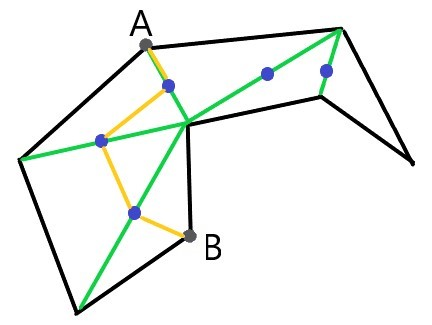
\includegraphics[scale=0.6]{segment_images/arc}}
			\caption{дуга АВ (желтый цвет), проведенная в многоугольнике}
			\label{arc}
		\end{minipage}
		\hfill
		\begin{minipage}[h]{0.4\linewidth}
			\center{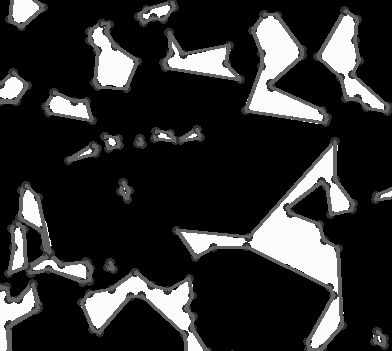
\includegraphics[scale=0.7]{segment_images/lines_resized}}
			\caption{Выделенные регионы связующего вещества с линиями периметра (серые прямые)}
			\label{fig:find_contour}
			\end{minipage}
		\end{center}
	\end{figure}


	 

	 \newpage
	 \section{Сбор геометрии}
	 
	 \subsection{Распределение углов}
	 
	 Принцип работы алгоритма выделения контура \ref{fig:find_contour} основан на проходе границы региона связующего вещества матрицей свертки по часовой стрелке (рис. \ref{clock}).
	 
	 На этом основан наш способ подсчёта углов. Будем считать, что нам интересны <<внутренние>> углы --- на рисунке \ref{clock} они отмечены зелёным. <<Внешний>> угол можно получить если из $360^\circ$ вычесть внутренний угол.
	 
	 
	 
	  \begin{figure}[h]
	 	\center{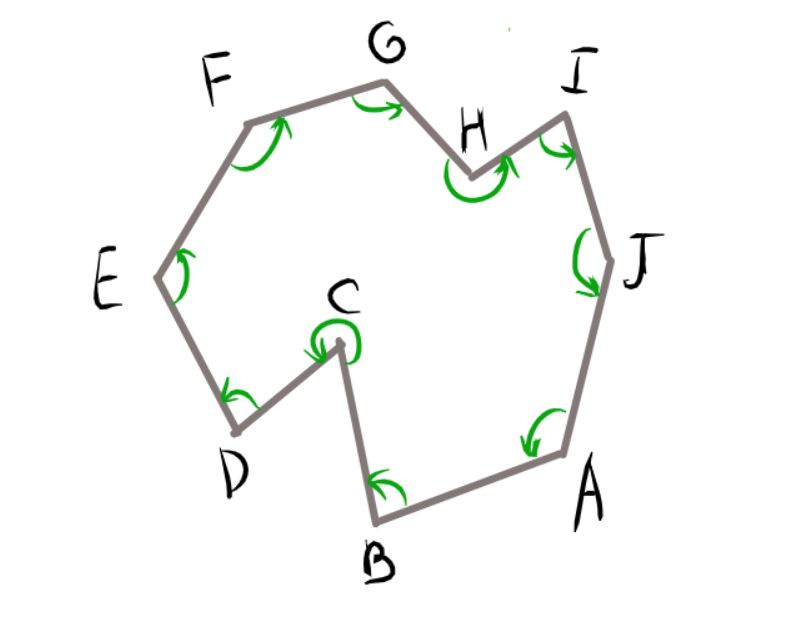
\includegraphics[scale=0.6]{segment_images/1.JPG}}
	 	\caption{направление обхода контура}
	 	\label{clock}
	 \end{figure}
	 
	 
	 \begin{figure}[h]
	 	\begin{center}
	 		\begin{minipage}[h]{0.4\linewidth}
	 			\center{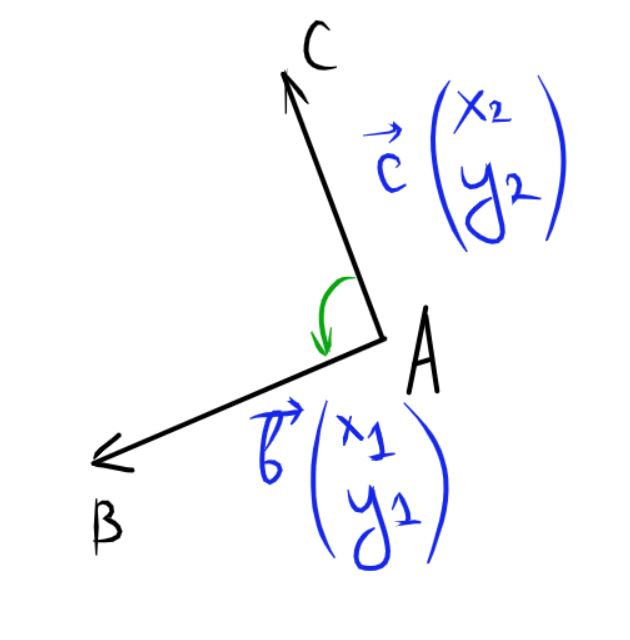
\includegraphics[scale=0.4]{segment_images/2.JPG}}
	 			\caption{пара векторов}
	 			\label{duo}
	 		\end{minipage}
	 		\hfill
	 		\begin{minipage}[h]{0.4\linewidth}
	 			\center{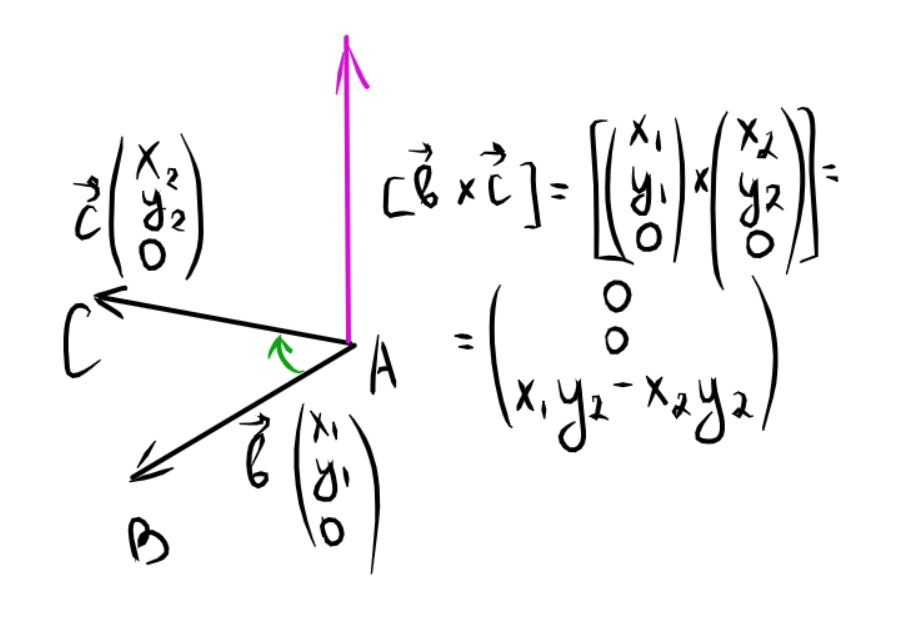
\includegraphics[scale=0.4]{segment_images/3.JPG}}
	 			\caption{тройка векторов}
	 			\label{trio}
	 		\end{minipage}
	 	\end{center}
	 \end{figure}
 
 	
 	Заметим, что нас интересует угол между векторами против часовой стрелки.
 	
 	Рассмотрим вектора $\overrightarrow b$ и $\overrightarrow c$ с координатами $(x_1, y_1)$ и $(x_2, y_2)$ соответственно (рис. \ref{duo}).
 	Угол между векторами $\alpha$:
 	
 	$$\alpha = \frac{(\overrightarrow b, \overrightarrow c)}{|\overrightarrow b||\overrightarrow c|} \cdot \frac{180^\circ}{\pi}$$
 	
 	Однако в данном случае мы получим угол от $0^\circ$ до $180^\circ$. В нашей постановке задачи это нас не устраивает --- мы же хотим отличать внутренние углы от внешних. 
 	
 	
 	
 	
 	
 	Для того чтобы узнать направление полученного угла мы воспользуемся векторным произведением (рис. \ref{trio}). (Допишем третью нулевую координату векторам). Вектор, получившийся в результате векторного произведения будет образовывать с векторами $\overrightarrow b$ и $\overrightarrow c$ правую тройку. Таким образом мы и определяем какой угол нас интересует - $\alpha$ или $360^\circ - \alpha$. 
 	
 	
 	Видим, что на самом деле направление угла определеляет знак определителя:
 	
 	\begin{equation*}
 		D = \left|
 		\begin{array}{cccc}
 			x_1 & x_2 \\
 			y_1 & y_2 
 		\end{array}
 		\right|
 	\end{equation*}
 	
 	Если $D >=0$, то искомый угол равен $\alpha$, если $D < 0$, то искомый угол $360^\circ - \alpha$.
 	
 	\subsection{Распределение диаметров}
 	
 	Диаметром пустоты будем называть диаметр окружности с наименьшим радиусом, в которую можно вписать пустоту.
 	
 	Пока что мы принимаем за диаметр максимальное расстояние между точками многоугольника.
 	
 	\begin{figure}[h]
 		\begin{center}
 			\begin{minipage}[h]{0.4\linewidth}
 				\center{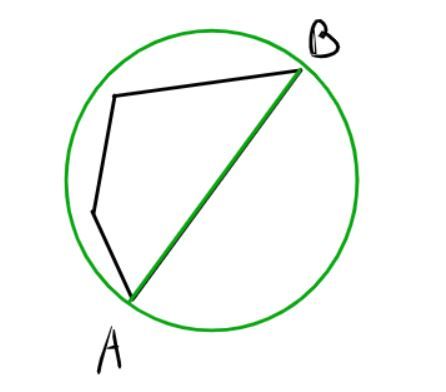
\includegraphics[scale=0.7]{segment_images/4.JPG}}
 				%\caption{}
 				%\label{ris:noise}
 			\end{minipage}
 			\hfill
 			\begin{minipage}[h]{0.4\linewidth}
 				\center{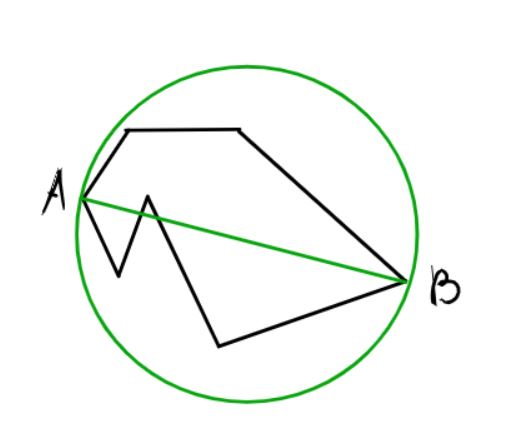
\includegraphics[scale=0.7]{segment_images/5.JPG}}
 				%\caption{}
 				%\label{fig:combine2}
 			\end{minipage}
 		\end{center}
 	\end{figure}
 	
 	
 	Тем не менее этот способ не всегда рабочий. Пример:
 	
 	
 	\begin{figure}[h]
 		\center{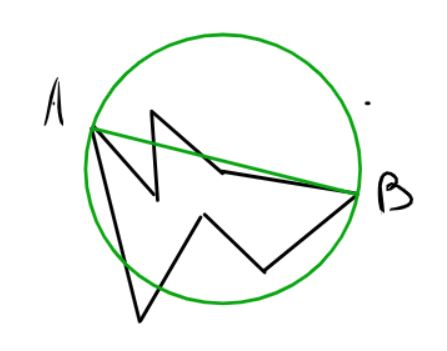
\includegraphics[scale=0.7]{segment_images/6.JPG}}
 		\caption{пример неверного определение диаметра }
 		\label{marked}
 	\end{figure}
 	
 	
 	Над этим ещё нам предстоит поработать.


	 
		
	\subsection{Распределение дуг}
	
	Пусть нужно провести дугу из первого угла региона во второй. Для этого нужно реализовать следующую последовательность алгоритмов 
	\begin{itemize}
		\item триангуляция многоугольника;
		
		\item поиск точек медиан на сторонах треугольников, которые находятся внутри региона;
		
		\item создание графа из точек медиан и соединение их ребрами 
		
		\item поиск кратчайшего пути в графе из исходной вершины угла в заданную.
	\end{itemize}
	
	
	

\section{Выводы}



\newpage
%далее сам список используевой литературы
\begin{thebibliography}{}
	
	
		\bibitem{find_contour}  Satoshi Suzuki,Keiichi Abe   -  \href{https://www.sciencedirect.com/science/article/abs/pii/0734189X85900167}{Topological Structural Analysis of Digitized Binary Images by Border Following}
	
	

		


\end{thebibliography}
	



	
\end{document}